\documentclass{article}
\usepackage{ragged2e}
\usepackage{wasysym}
\usepackage{amsmath}
\usepackage{graphicx} % Required for inserting images
\usepackage{listings} % Code 
\usepackage{fancyhdr}
\usepackage{hyperref}
\usepackage{wrapfig}
\usepackage{amssymb}
\usepackage[utf8]{inputenc}
\usepackage[T1]{fontenc}
\usepackage{geometry}
\usepackage{graphicx}
\usepackage{tikz}
\usetikzlibrary{positioning}
\usetikzlibrary{calc}
\usepackage{graphicx}
\usepackage{tocloft}
\usepackage{subcaption}

\hypersetup{
    colorlinks=true,
    linkcolor=blue,
    filecolor=magenta,
    urlcolor=cyan,
}
\begin{document}
\begin{titlepage}
\centering
%\pagecolor{yellow}
\vspace{5cm}

\textbf{\Huge Large Language Models} \\
\vspace{0.5cm}
\textbf{\Large MID SUMMER REPORT} \\
\vspace{0.5cm}
\textbf{\Large Aditya Singh}\\
\vspace{0.5cm}
\textbf{\Large Roll Number: 22B1844}\\
\vspace{0.5cm}
\textbf{\Large Mentor: Parth Pai}\\
\vspace{0.5cm}
\textbf{\Large Summer of Science 2024} \\
\vspace{1cm}


\includegraphics[width=0.45\textwidth]{Robot mic.png} \\
\vspace{0.5cm}

\includegraphics[width=0.45\textwidth]{Featured-Blog-Image-A-Comprehensive-Overview-of-Large-Language-Models-1024x768.jpg}


\end{titlepage}

\clearpage

\tableofcontents

\newpage

\section{\Huge {Introduction}}

\vspace{0.4cm}
\flushleft
\Large
\justifying
For the first half of the project we study Natural Language Processing concepts and in the next half we will dive into concepts related to Large Language Models.

\section{\Huge Recurrent Neural Networks(RNNs)}
Natural Language Processing requires understanding the meaning of the whole sequence of words present in the text. This cannot be done by the classical neural networks. For this we use a different type of networks called RNNs.

\flushleft
RNNs are sequential networks in which in the forward pass information gained from earlier in the sequence is passed forward. This way the network is able to use information from earlier to get the context later.
\vspace{.5cm}

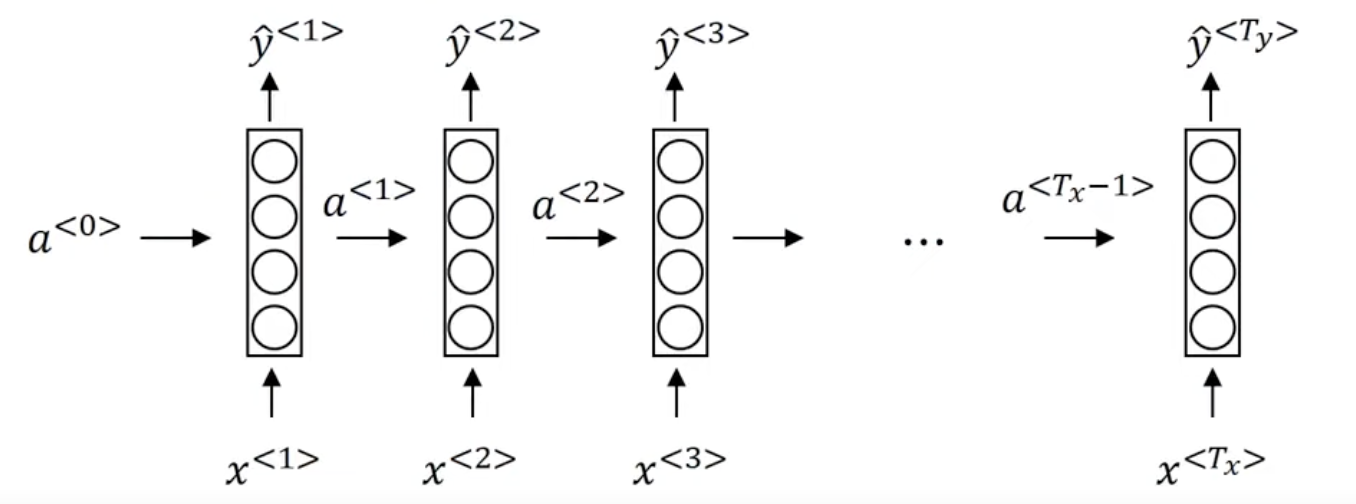
\includegraphics[width= 1\textwidth]{2.png} \\
\vspace{.5cm}
The above diagram shows the structure of RNN networks.

\newpage
The equations involved are:
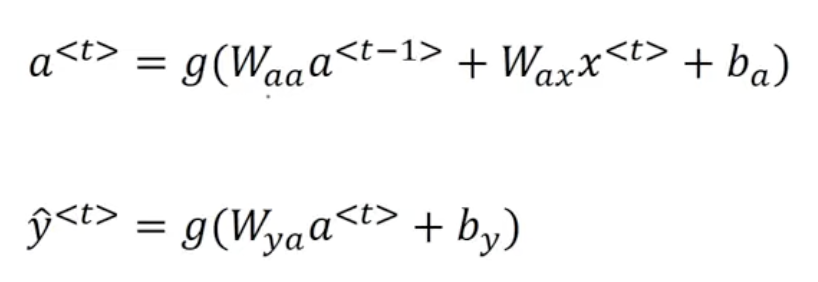
\includegraphics[width=.9\textwidth]{1.png}

One of the uses of RNNs is Named Entity Recognition, in the network identifies the names of objects.

\section{\Huge Representation of Words}
Words are represented using One-Hot notations. We take a vocabulary of all words V. Each word is represented by a vector of number of dimensions equal to the size of V. All the elements of the vector are 0 except one which corresponds to the index of the word being represented.

\section{\Huge Language Modelling}
Language modeling involves predicting the next word in a sequence based on the words that precede it. This is fundamental in NLP, as it helps machines understand and generate human language. Modern models, such as GPT, utilize deep learning and vast datasets to achieve remarkable accuracy and fluency in text generation.

\section{\Huge Vanishing Gradient Problem in RNNs}
Vanishing gradients in recurrent neural networks (RNNs) occur when gradients used for updating the network's weights diminish exponentially during backpropagation. This makes it difficult for the model to learn long-term dependencies, as the weights associated with distant past inputs receive minimal updates. Techniques like Long Short-Term Memory (LSTM) and Gated Recurrent Units (GRUs) help mitigate this issue.

\section{\Huge Gated Recurrent Units(GRUs)}
Gated Recurrent Units (GRUs) are a type of recurrent neural network designed to address the vanishing gradient problem. GRUs use gating mechanisms to control the flow of information, enabling them to capture long-term dependencies more effectively. They combine the input and forget gates into a single update gate, simplifying the architecture and improving training efficiency compared to traditional RNNs.


\section{\Huge Long Short Term Memory Units(LSTMs)}
Long Short-Term Memory (LSTM) networks are an advanced type of recurrent neural network (RNN) designed to better capture long-term dependencies in sequential data. They use special units called memory cells, which can maintain information over long periods. LSTMs employ three gates—input, forget, and output—to regulate the flow of information, making them highly effective at handling vanishing gradient issues and learning from long sequences. \\

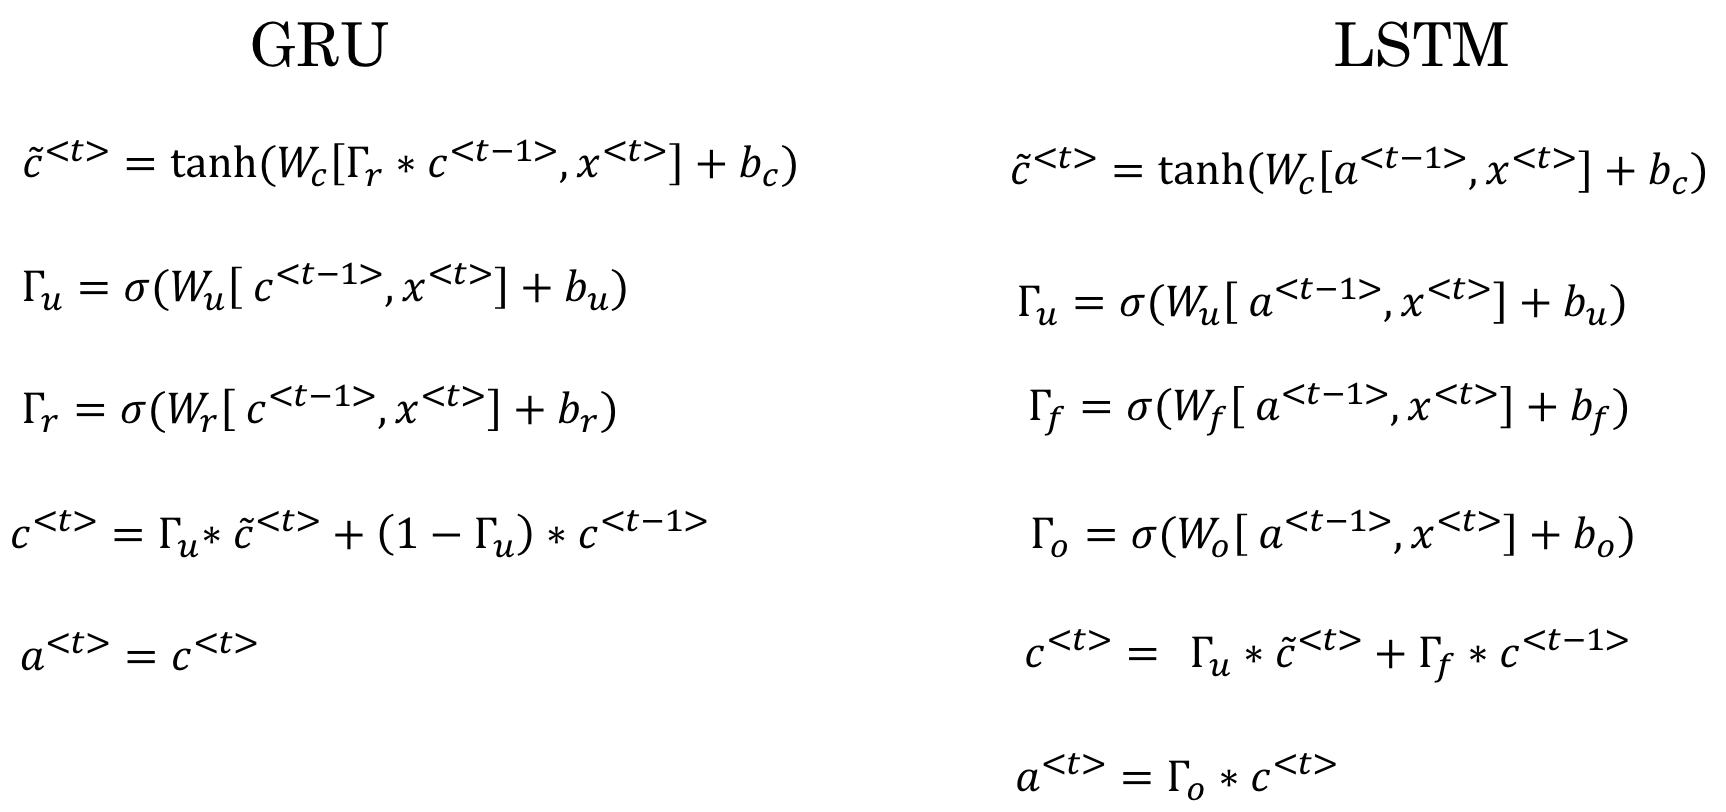
\includegraphics[width=.9\textwidth]{3.png}

The below image shows the structure of LSTMs.
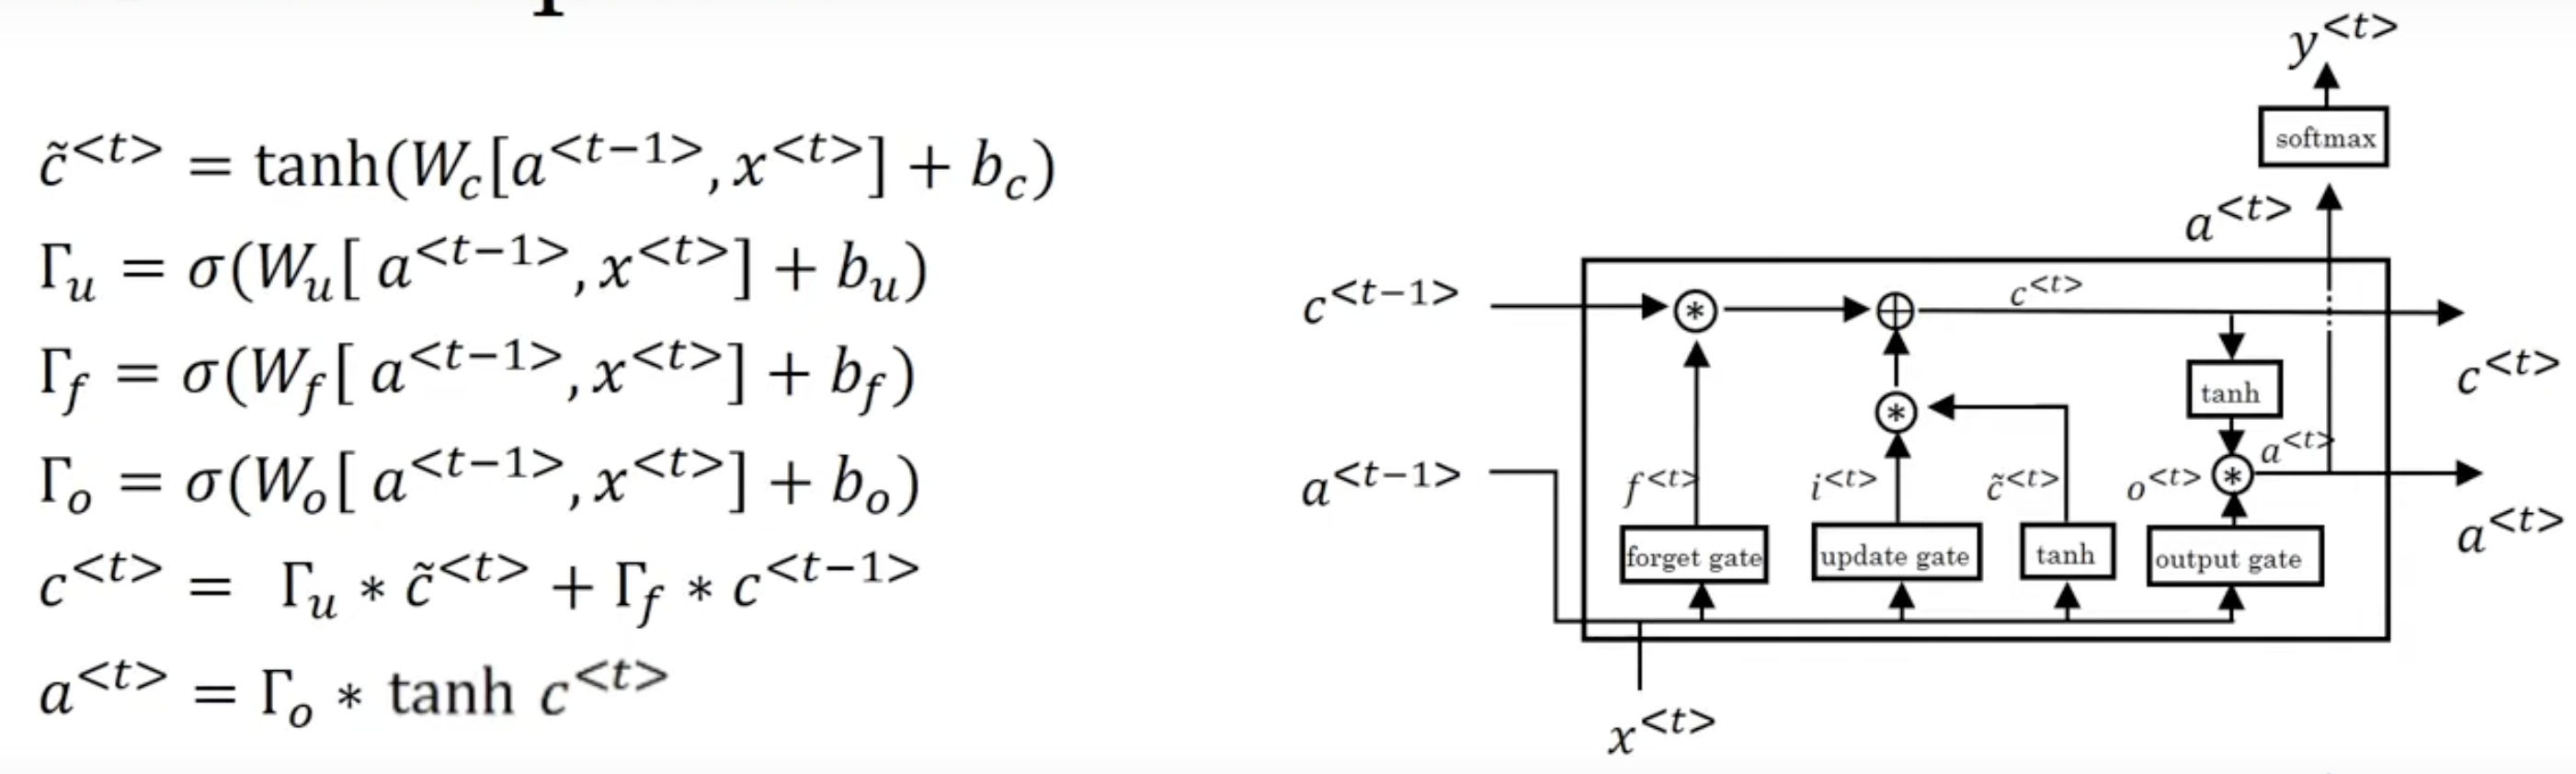
\includegraphics[width=.9\textwidth]{4.png}


\section{\Huge Bidirectional RNNS(BRNNs)}
Bidirectional Recurrent Neural Networks (BRNNs) enhance the learning capability of standard RNNs by processing data in both forward and backward directions. This structure allows BRNNs to capture context from both past and future states simultaneously, providing a more comprehensive understanding of the sequence. This bidirectional approach is particularly useful for tasks like speech recognition and machine translation, where context from both directions is crucial.

\section{\Huge Word Embeddings}
Now we study another way to represent words. We use feature vectors for each word, i.e. we decide certain features and each word is represented by a vector of size equal to teh number of features. So each word is basically a point in an n-dimensional space where n is the number of features.

\flushleft
This representation is quite useful to capture relations between different words. It makes it easier to find analogies. For example, $v_{\text{king}} - v_{\text{man}} + v_{\text{woman}} = v_{\text{queen}}$

\section{\Huge Embedding Matrix}
An embedding matrix is a trainable parameter matrix used in neural networks to store word embeddings. Each row corresponds to the vector representation of a word in the vocabulary. During training, the embedding matrix is updated to capture semantic information from the context in which words appear. This matrix transforms input words into dense vectors, enabling models to process and understand text more effectively. It is essential in tasks like text classification, translation, and sentiment analysis, as it provides meaningful word representations that improve the overall performance of the model.

\section{\Huge Word2Vec and GloVe}
Word2Vec and GloVe are two popular techniques for generating word embeddings.
Word2Vec, developed by Google, uses neural networks to learn word associations from large text corpora. It has two main models: Continuous Bag of Words (CBOW) and Skip-gram. CBOW predicts a target word from its context, while Skip-gram predicts the context given a target word.
GloVe (Global Vectors for Word Representation), developed by Stanford, leverages word co-occurrence statistics from a corpus. It builds a word-word co-occurrence matrix and derives embeddings by factorizing this matrix, ensuring that similar words have similar vector representations.
Both methods produce dense, continuous vector representations that capture semantic relationships between words, enhancing various NLP tasks.

\section{\Huge Sentiment Analysis}
Sentiment classification involves determining the emotional tone behind a piece of text, such as identifying whether a movie review is positive or negative. It uses natural language processing techniques to analyze and categorize text based on sentiment. Models often use word embeddings to represent text and neural networks like RNNs, LSTMs, or transformer-based models (e.g., BERT) to learn sentiment patterns. This classification is crucial for applications like customer feedback analysis, social media monitoring, and market research, enabling businesses to gauge public opinion and make data-driven decisions.

\section{\Huge Debiasing word embeddings}
Debiasing word embeddings is a process that aims to mitigate biases present in the vector representations of words. Biases can stem from the data used to train embeddings, reflecting societal biases and stereotypes. Techniques such as neutralizing, which removes gender or other biased associations from word embeddings, and equalizing, which modifies embeddings to have equal representation across sensitive attribute groups, help address these issues. Debiasing is crucial for fair and unbiased NLP applications, promoting ethical AI development and mitigating potential harm caused by biased language models.

\section{\Huge Attention Model}
Attention models are a type of neural network architecture that focuses on learning which parts of input data are relevant at each step of computation. Originally used in sequence-to-sequence tasks like machine translation, attention mechanisms allow models to weigh the importance of different input elements dynamically, rather than treating them equally throughout processing. This results in improved performance by enabling the model to focus more on relevant information, making attention models particularly effective for tasks involving long sequences or complex data relationships.

\section{\Huge Speech Recognition}
Speech recognition is the process of converting spoken language into text or commands that a computer can understand and process. It involves several stages:
\begin{enumerate}
    \item Audio Preprocessing: The incoming audio signal is filtered and transformed into a format suitable for analysis.
    \item Feature Extraction: Features like Mel Frequency Cepstral Coefficients (MFCCs) are extracted from the audio to capture relevant information.
    \item Acoustic Modeling: A model, often based on deep learning (e.g., Convolutional Neural Networks or Recurrent Neural Networks), learns to map audio features to phonemes or basic speech units.
    \item Language Modeling: Another model predicts the likelihood of word sequences based on their context, improving accuracy by incorporating linguistic knowledge.
    \item Decoding: The models work together to transcribe the audio into text, with techniques like beam search or dynamic programming used to find the most likely sequence of words.
    \item Modern speech recognition systems, such as those used in virtual assistants like Siri or Google Assistant, leverage large datasets, deep learning techniques, and language models to achieve high accuracy and handle diverse accents and languages.
\end{enumerate}

\section{\Huge Transformers}
Transformers are a groundbreaking type of deep learning model primarily used in natural language processing (NLP) tasks. Unlike traditional sequence models like RNNs or LSTMs, transformers rely entirely on attention mechanisms to draw global dependencies between input and output elements in parallel, making them highly efficient for processing long sequences. The transformer architecture consists of an encoder-decoder framework, with multiple layers of self-attention and feedforward neural networks. Transformers have revolutionized NLP with models like BERT, GPT, and T5, achieving state-of-the-art performance in tasks such as language translation, text generation, sentiment analysis, and question answering.

\section{\Huge Self Attention}
Self-attention is a key mechanism used in transformer-based neural networks, particularly in natural language processing (NLP) tasks. It allows the model to weigh the importance of different words in a sequence when processing the input.

Here's how self-attention works:
\begin{enumerate}
\item Input Embeddings: Each word in the input sequence is initially embedded into a vector representation.
\item Attention Scores: The self-attention mechanism calculates attention scores between each pair of words in the sequence. These scores determine how much focus each word should place on other words.
\item Attention Weights: The attention scores are normalized and used as weights to compute a weighted sum of the input embeddings, generating context-aware representations for each word.
\item Output: The context-aware representations are then passed through feedforward layers to produce the final output for the model.
\end{enumerate}
Self-attention enables transformers to capture long-range dependencies and semantic relationships within the input sequence, making them highly effective for tasks like machine translation, text summarization, and sentiment analysis.

\section{\Huge Multi-Head Attention}
Multi-head attention is an extension of the self-attention mechanism used in transformer architectures. It enhances the model's ability to capture diverse relationships within the input data by performing attention computations multiple times in parallel, each with different learned projections.

Multi-head attention works as follows:
\begin{enumerate}
\item Input Embeddings: Input sequences are embedded into vectors.
\item Multi-Head Projection: The input embeddings are linearly projected into multiple different spaces (heads) using learned weight matrices.
\item Scaled Dot-Product Attention: For each head, attention scores are computed between the projected query, key, and value vectors.
\item Attention Aggregation: The attention scores are scaled and used to weight the corresponding value vectors, which are then concatenated across all heads and linearly transformed to generate the multi-head attention output.
\item Final Output: The multi-head attention output is typically passed through another layer (e.g., feedforward network) for further processing.
\end{enumerate}
Multi-head attention allows the model to attend to different aspects of the input simultaneously, capturing complex relationships and improving performance on a wide range of NLP tasks.

\newpage

\begin{center}
    \section*{\Huge \underline{Revised Plan of Action}}
\end{center}

\vspace{0.5cm}

\begin{itemize}
    \Large
    \item \textbf{\Large Week5}: Introduction to Large Language Models, Decoding Strategies, Fine Tuning Pre-Trained LLMs
    \vspace{0.3cm}
    \item \textbf{\Large Week6}: Understanding Prompt Engineering, starting Multimodal Learning, Finishing Multi-Modal Learning and Understanding Retrieval Augmented Generation(RAG)
    \vspace{0.3cm}
    \item \textbf{\Large Week7}: Understanding the Langchain framework, RAG and LLaMa architectures
    \vspace{0.3cm}
    \item \textbf{\Large Week8}: Implementing a project using all the knowledge gained in the SOS project.(The exact detils will be decided later based on the material covered)
    \vspace{0.4cm}
    
    \begin{center}
        \textbf{\Large SOS FINAL REPORT SUBMISSION}
    \end{center}
\end{itemize}

\end{document}